% Atomic (linearizable) history from Fig.2 (b) of [Herlihy@TOPLAS'90],
% which is in turn from Fig. 3 of [Misra@TOPLAS'86].

\documentclass{standalone}

\usepackage{tikz}

\tikzset{wop/.style = {blue, very thick},
  rop/.style = {brown, very thick}}

% interval for operations
\newcommand{\itv}[5]{ % #1: start point; #2: end point; #3: operation name; #4: style; #name
  \coordinate (start #3) at #1;	% start point
  \coordinate (end #3) at #2;	% end point

  \draw[#4, |-|] (start #3) -- (end #3) % draw the interval
  node[pos = 0.5, above = 1mm, font = \Large] (#5) {\textsl{#3}}; % attach the operation name
}

\begin{document}
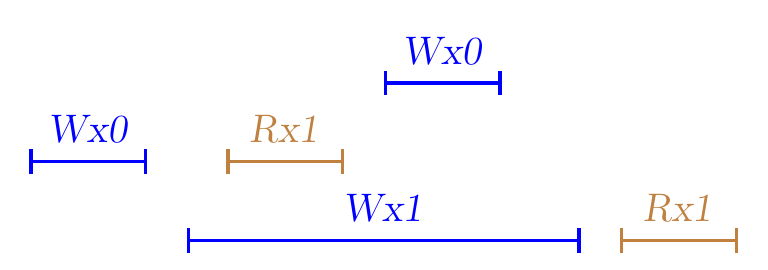
\begin{tikzpicture}
  \itv{(2,0)}{(7,0)}{Wx1}{wop}{wx1}
  \itv{(7.5,0)}{(9,0)}{Rx1}{rop}{rx1}

  \itv{(0,1)}{(1.5,1)}{Wx0}{wop}{wx0}
  \itv{(2.5,1)}{(4,1)}{Rx1}{rop}{rx1}

  \itv{(4.5,2)}{(6,2)}{Wx0}{wop}{wx0}
\end{tikzpicture}
\end{document}
